\section{Water tower time constant}
\label{sec:WT_TimeConstant}

\subsection*{Purpose:}
The purpose of this test is to determine the time constant and settling time of WT.


%\subsection{One clamp push} % \label{app:...}
\subsection*{Test equipment:}
\begin{itemize}
\item The water distribution system at AAU.
\end{itemize}

\subsection*{Procedure:}
The following procedure was made for finding the time constant:
\begin{enumerate}
\item Wait for the system to get into a steady state position with the following system setup: valve opening at $0.7 \%$ for all consumer valves and differential pressure over pumps at $C2 = C16 = 0.2 Bar$, $C18 = 0.1 Bar$, $C25 = 0.25 Bar$.
\item Increase the differential pressure over C2 with 0.1 Bar.
\item Wait 1.5 hour.
\end{enumerate}


\subsection*{Measuring data:}
The measurements data can be found on the attached storage under the path: \path{CD:/Data/WT timeconstant}, a plot of the data is shown in \figref{fig:Test_WT_Timeconstant}.

\subsection*{Results:}

The time constant of the WT can be found through the linear differential equation shown in \eqref{statespace_4}. By Laplace transform and solving for the input output relation, the standard form of the transfer function for the WT can be derived as see in \eqref{eq:std_trans_tank_time}

\begin{equation}
	\begin{split}
	&\Delta \dot{p}_{WT} = A_p \Delta \hat{p}_{WT}  + \pmb{B_p}\pmb{\hat{u}}\\
	&s\Delta p_{WT}(s) = A_p \Delta \hat{p}_{WT}(s)  + \pmb{B_p}\pmb{\hat{u}(s)}\\
	&\frac{\Delta p_{WT}(s)}{u(s)} = \frac{B}{s-A} = \frac{\frac{B}{A}}{\frac{1}{A}s + 1}
	\end{split}
	\label{eq:std_trans_tank_time}
\end{equation}

From the denominator, the time constant of the WT can be directly read as seen in \eqref{eq:direct_time_constant}

\begin{equation}
	\tau s + 1
	\label{eq:direct_time_constant}
\end{equation}

Since A in \eqref{statespace_4} is a constant, due to the tank only having one state, the WT has one time constant. However the unit of A is in $[\frac{m^3}{h}]$ and needs to be convert to seconds. 

As the dynamics of the WT are described by a first order system, the time constant can be found as the time the system uses to reach $63.2\%$ of the steadystate pressure.
This pressure at $63.2\%$ of the steadystate values is based on the minimum and maximum pressure values during the step and determined to:

\begin{equation}
(0.137 - 0.127)*63.2 \% = 0.0063 \rightarrow 0.127 + 0.0063 = 0.133 Bar 
\end{equation}

Based on the data is it found that at a pressure of 0.133 bar the time is passed is 1155 seconds corresponding to 19,25 minutes. 

On \figref{fig:Test_WT_Timeconstant} the measurement data used to determine the time constant of the WT is shown. A small red dot indicates the time constant for the tank.

\begin{figure}[H]
% This file was created by matlab2tikz.
%
%The latest updates can be retrieved from
%  http://www.mathworks.com/matlabcentral/fileexchange/22022-matlab2tikz-matlab2tikz
%where you can also make suggestions and rate matlab2tikz.
%
\definecolor{mycolor1}{rgb}{0.00000,0.44700,0.74100}%
%
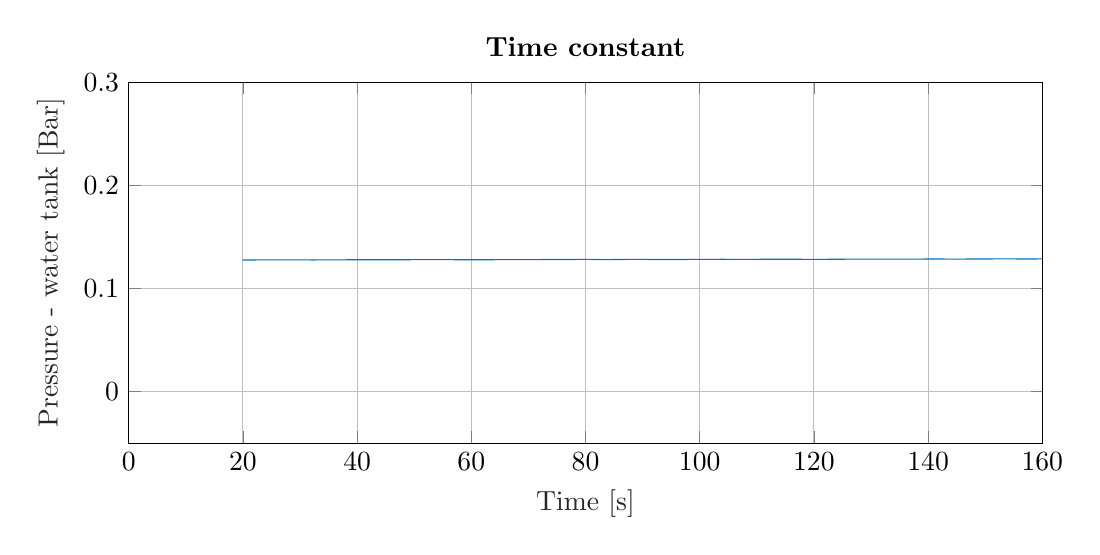
\begin{tikzpicture}

\begin{axis}[%
width=4.568in,
height=1.803in,
at={(0.766in,0.486in)},
scale only axis,
xmin=0,
xmax=160,
xlabel style={font=\color{white!15!black}},
xlabel={Time [s]},
ymin=-0.05,
ymax=0.3,
ylabel style={font=\color{white!15!black}},
ylabel={Pressure - water tank [Bar]},
axis background/.style={fill=white},
title style={font=\bfseries},
title={Time constant},
xmajorgrids,
ymajorgrids,
legend style={legend cell align=left, align=left, draw=white!15!black}
]
\addplot [color=mycolor1, forget plot]
  table[row sep=crcr]{%
19.9499999999998	0.127718914955949\\
28.3999999999996	0.127870293255\\
32.3000000000002	0.127749364613919\\
41.5	0.127992961876771\\
44.5	0.127931192570941\\
53.6499999999996	0.128068651026297\\
61.8500000000004	0.127909442815508\\
66.8500000000004	0.128131290322926\\
69.1000000000004	0.12808866080195\\
80.6000000000004	0.128282668621978\\
83.1499999999996	0.128073870967455\\
88.8000000000002	0.128322688172375\\
93.8500000000004	0.128142600195133\\
104	0.128398377321901\\
107.15	0.128318338221106\\
115.7	0.128489726294902\\
119.95	0.128293108504295\\
129.2	0.128623704789788\\
131.5	0.128509736070555\\
142.3	0.128676774193991\\
143.7	0.128563675464648\\
154.75	0.128808142717389\\
155.95	0.128657634408228\\
167.2	0.128916891495464\\
175.55	0.128753333333407\\
181.9	0.128791612903115\\
186.8	0.129037820136546\\
191.75	0.128879481915646\\
194.45	0.129044780058393\\
211	0.128913411534995\\
216.05	0.129144828934841\\
221.7	0.128929071358471\\
226.7	0.12920833822136\\
228.6	0.129100459433175\\
230.85	0.129271847506971\\
241.5	0.129193548386866\\
249	0.12946063538584\\
254.5	0.129156138807048\\
264.05	0.129474555229535\\
271.6	0.12933361681371\\
275.05	0.12949108504381\\
277.5	0.12939886608001\\
289.7	0.129556334311019\\
294.55	0.129502394916926\\
298.25	0.129668563049563\\
302.25	0.12952066471189\\
314.1	0.129822551320103\\
319.1	0.129589393939568\\
324.05	0.129951309872922\\
328.95	0.129683352884058\\
333.8	0.129859090909122\\
339.5	0.129862570869591\\
346.05	0.129699012707533\\
351.45	0.129711192570539\\
356.4	0.130098338220705\\
369.9	0.129883450635134\\
375.6	0.130079198435851\\
381.85	0.129915640273794\\
386.85	0.130286256109684\\
388.5	0.130033958944296\\
399.1	0.130234926686171\\
402.55	0.130102688171974\\
411.7	0.130407184750766\\
417.4	0.130193167155085\\
419.55	0.130397614858339\\
425.6	0.130256676441604\\
434.35	0.13039326490707\\
437.05	0.130321055718923\\
447.65	0.130566392961555\\
451.65	0.130488963832249\\
460.1	0.130624682306916\\
466.15	0.130478523949023\\
473.35	0.130796070381621\\
473.7	0.130752570869845\\
478.2	0.130481133919602\\
489.4	0.13061076246322\\
498.2	0.130820430107633\\
504	0.130729951124522\\
508.55	0.130930048875598\\
512.95	0.130970068425995\\
519.1	0.130730821114412\\
525.65	0.130803900293358\\
530.6	0.131157116324175\\
535.1	0.130907429130275\\
546.8	0.131124056695626\\
551.7	0.131219755620805\\
558.4	0.131050977516679\\
562.15	0.131033577712515\\
571.8	0.131405933529095\\
571.85	0.131416373411412\\
580.15	0.131068377321753\\
584.15	0.131133626588053\\
589.75	0.131437253176955\\
605.05	0.131238025415769\\
607.15	0.1314842326492\\
612.15	0.1312989247308\\
619.85	0.131537302052493\\
624.85	0.131369393939167\\
629.85	0.131599941349123\\
633.150000000001	0.131387663734131\\
645.3	0.131637350928941\\
647.2	0.131740879764948\\
651	0.131458132942498\\
667.3	0.13160777126086\\
669.900000000001	0.131782639296034\\
674.45	0.131666060606221\\
681.55	0.13188790811364\\
684.900000000001	0.1318270087977\\
686.55	0.131565141739884\\
695.400000000001	0.131720869990204\\
700.400000000001	0.131909657869073\\
706.75	0.131805259042267\\
711.35	0.131961857282477\\
726.05	0.132121065493266\\
731.05	0.131787859237193\\
731.2	0.131800039101108\\
743.35	0.132049726295008\\
750.95	0.131927927664037\\
755.45	0.132256783968842\\
756.3	0.132289843597391\\
759.75	0.13198273704802\\
773.95	0.132395112414088\\
778.150000000001	0.132116715542907\\
780.6	0.132309853372135\\
792.5	0.132134985336961\\
801.95	0.132547360703938\\
804.75	0.132431652004016\\
806.95	0.132198494623481\\
817.5	0.132232424242829\\
827.45	0.132437741935064\\
834.150000000001	0.132599560117342\\
839.75	0.132309853372135\\
848.400000000001	0.132507341153541\\
853.05	0.132371622677965\\
854.05	0.132411642228362\\
861.150000000001	0.132749198435704\\
866.150000000001	0.132496901270315\\
869.05	0.132652629520635\\
879.5	0.132493421309846\\
887.35	0.132757028348351\\
892.35	0.132500381231694\\
901.1	0.132742238513856\\
903.85	0.132777908112985\\
911.8	0.132675249266867\\
916.8	0.13275963831893\\
921.85	0.132647409579477\\
931.8	0.132896226784396\\
933.25	0.132739628543277\\
939.900000000001	0.132764858260089\\
949.900000000001	0.133011935484319\\
955.150000000001	0.132806617791175\\
961.650000000001	0.133022375366636\\
966.95	0.132876217008743\\
975.1	0.13313373411529\\
980.45	0.133171143695108\\
985.45	0.132911016617982\\
989.400000000001	0.132985835776708\\
999.650000000001	0.133281632453873\\
1004.3	0.132994535679245\\
1007.95	0.133274672532025\\
1019.15	0.133239872922786\\
1024.3	0.133081534701887\\
1034	0.13304238514138\\
1036.75	0.133443450635241\\
1038.9	0.133367761485715\\
1041.8	0.133138084066559\\
1051.95	0.133385161290789\\
1057.75	0.133260752688329\\
1063.5	0.13353827956962\\
1068.55	0.133292942326079\\
1074.95	0.133329481916007\\
1082.4	0.133692267839251\\
1087.35	0.133318172042891\\
1094.9	0.133549589442737\\
1103.9	0.133408651026002\\
1109	0.133685307918313\\
1114	0.13344606060582\\
1116.4	0.133673998045197\\
1130.75	0.133674868035087\\
1133.2	0.133519139784767\\
1136.05	0.133553069404115\\
1144	0.133811456500553\\
1149	0.133574819159548\\
1159.65	0.133770566960266\\
1164.2	0.133745337243454\\
1169.55	0.133608748777988\\
1173.75	0.133660078201501\\
1175.9	0.133905415445042\\
1186.4	0.133737507331716\\
1196.5	0.133878445747541\\
1204.8	0.134064623655831\\
1209.45	0.133777526882113\\
1209.8	0.133747077224143\\
1218.15	0.133990674486995\\
1221.7	0.133816676441711\\
1233.9	0.134023734115544\\
1242.9	0.133934995112213\\
1244.4	0.134175982404486\\
1249.4	0.133894975561816\\
1258.45	0.134182072336444\\
1259.15	0.134247321602743\\
1264.25	0.133981974584458\\
1271.35	0.134030694037392\\
1282.85	0.134216001954883\\
1291.3	0.134028084066813\\
1293.2	0.134305610948104\\
1298.15	0.133990674486995\\
1302.25	0.134279511241402\\
1307.65	0.134124652981882\\
1319.05	0.134486568915236\\
1319.9	0.134358680352307\\
1324.05	0.134143792766736\\
1334.25	0.134156842619632\\
1339.85	0.134337800586763\\
1347.75	0.134490048875705\\
1353	0.134152492668363\\
1363.6	0.134295171065787\\
1368.6	0.1345039687194\\
1371.95	0.13453441837737\\
1376.75	0.134256891496079\\
1389.4	0.134574437927768\\
1393.2	0.134363900293465\\
1394.55	0.134326490713647\\
1405.3	0.134553558162224\\
1406.1	0.134559648094182\\
1412.7	0.134374340175782\\
1420.9	0.134419579667338\\
1425.55	0.134711026393234\\
1436.2	0.134783235581381\\
1441.2	0.134448289344618\\
1448.85	0.13456660801603\\
1454.65	0.134738866079715\\
1460.5	0.13462837732186\\
1462.5	0.134799765395655\\
1467.9	0.134843264907431\\
1477.55	0.134634467252909\\
1480.3	0.134805855327613\\
1489.9	0.134616197458854\\
1495.95	0.134928523949384\\
1501.4	0.134671876832726\\
1504.2	0.134849354838479\\
1509.8	0.134714506353703\\
1517.75	0.134740606060404\\
1526.9	0.135005953079599\\
1530	0.134918084066157\\
1531.95	0.13469362658816\\
1540.75	0.134775405669643\\
1550.9	0.134918084066157\\
1558.15	0.134783235581381\\
1560.35	0.134967673508982\\
1566.1	0.134818905180509\\
1572.1	0.134975503421629\\
1581.3	0.135209530792054\\
1586.25	0.134798895405766\\
1590.4	0.134943313782969\\
1596.65	0.135112091886185\\
1602.45	0.134892854350255\\
1604.2	0.135112091887095\\
1616.05	0.135115571847564\\
1626.35	0.134953753665286\\
1626.95	0.134930263930073\\
1637.2	0.135165161290388\\
1640.3	0.135013782991336\\
1645.65	0.135206050830675\\
1654.35	0.135296529814696\\
1658.8	0.134992903225793\\
1669.6	0.135092082111441\\
1675.4	0.135224320625639\\
1683.15	0.135367869012953\\
1687.5	0.135085122189594\\
1688.05	0.135039012708148\\
1692.85	0.135360909091105\\
1703.75	0.135136451613107\\
1706.95	0.135362649071794\\
1719.8	0.135139931573576\\
1724.45	0.135341769306251\\
1725.05	0.135373088954111\\
1732.65	0.135213010752523\\
1739.4	0.135400928641502\\
1744.4	0.135254770283609\\
1754.15	0.135477487780918\\
1760.9	0.135268690127305\\
1768.1	0.135353079178458\\
1770.15	0.135214750733212\\
1778.4	0.135492277614503\\
1783.55	0.135291309872628\\
1789.05	0.135596676442219\\
1794.2	0.135214750733212\\
1804.85	0.135197350929047\\
1809.9	0.135512287390156\\
1811.5	0.135429638318783\\
1829.45	0.135685415444641\\
1834.8	0.135430508308673\\
1844.25	0.135392228738965\\
1846.75	0.135592326490951\\
1849.8	0.135606246334646\\
1857.75	0.135474877810339\\
1863.75	0.135637565982506\\
1865.8	0.135487927664144\\
1876	0.135692375366489\\
1879.9	0.135525337243052\\
1885.05	0.135520987292693\\
1891.25	0.13574979472105\\
1899.6	0.135804604105942\\
1902.25	0.135578406647255\\
1911.9	0.135808954056301\\
1916.95	0.135503587487619\\
1920.65	0.135567096774139\\
1932.75	0.135801994135363\\
1933.3	0.135834183773113\\
1939.55	0.135646265885043\\
1947.9	0.135835923753802\\
1956.8	0.135634086021128\\
1958.6	0.135652355816092\\
1966.9	0.135828093842065\\
1969.95	0.135722825024459\\
1981.3	0.135884643206737\\
1983.9	0.135953372434415\\
1986.6	0.135792424242027\\
2001.9	0.135930752688182\\
2004	0.135761104594167\\
2012.2	0.135743704790002\\
2017.4	0.135955112414194\\
2022.25	0.135745444770691\\
2029.95	0.135939452590719\\
2032.8	0.135822003910107\\
2040.15	0.136002961877239\\
2049.45	0.135808084066412\\
2054.6	0.135986432062964\\
2055.85	0.135879423264669\\
2060.15	0.13603167155452\\
2068.05	0.136083000978033\\
2074.55	0.1358750733134\\
2080.7	0.135967292277201\\
2083.1	0.135862023460504\\
2093.8	0.135866373411773\\
2099.35	0.136057771261221\\
2111.2	0.136095180841039\\
2116	0.135820263929418\\
2121	0.136052551320063\\
2125.9	0.13593771261003\\
2135.35	0.135898563049523\\
2141.4	0.136134330400637\\
2146.5	0.135865503420973\\
2153.75	0.135921182795755\\
2161.7	0.136103880742667\\
2174.7	0.136163910068717\\
2176.4	0.13593858259992\\
2179.2	0.135975122189848\\
2187.85	0.136149990225022\\
2192	0.135980342131006\\
2199	0.136246559140091\\
2204	0.135978602150317\\
2214.5	0.136221329423279\\
2215	0.136210889540962\\
2220.15	0.136046461388105\\
2233.75	0.136136070381326\\
2238.75	0.136024711632672\\
2239.9	0.136045591398215\\
2248	0.136262218963566\\
2254.3	0.136203929619114\\
2262.05	0.136039501466257\\
2266.35	0.136171739980455\\
2274.6	0.136045591398215\\
2278.8	0.136015141740245\\
2283.4	0.136253519061938\\
2288.55	0.136096050830929\\
2293.1	0.136228289345127\\
2301	0.136126500488899\\
2310.5	0.13624916911067\\
2315.2	0.136412727272727\\
2320.2	0.136103010752777\\
2330.95	0.136123020527521\\
2336.95	0.136348347996318\\
2345.75	0.136337908113092\\
2348.55	0.136158690126649\\
2353.45	0.13640663734077\\
2358.45	0.136182179862772\\
2362.5	0.136338778103891\\
2374.2	0.136159560117449\\
2374.4	0.136179569892192\\
2382.65	0.136451006842435\\
2387.65	0.136118670576252\\
2398.3	0.136440566960118\\
2404.35	0.136445786901277\\
2409.3	0.136235249266974\\
2415.85	0.136454486803814\\
2422.2	0.136209149560273\\
2423.55	0.136232639296395\\
2430.55	0.136443176930698\\
2435.85	0.136294408602225\\
2442	0.136524086021382\\
2447.95	0.136306588465231\\
2450.75	0.136463186705441\\
2463.95	0.13631180840639\\
2472.45	0.136596295210438\\
2477.3	0.136274398827481\\
2488.1	0.136501466276059\\
2493.85	0.136337038123202\\
2502.95	0.136346608015629\\
2509.25	0.136525826002071\\
2513.4	0.136634574780146\\
2518.4	0.136277008798061\\
2522.6	0.136444046920587\\
2529.15	0.136588465297791\\
2535.55	0.136396197458453\\
2546.05	0.136609345063334\\
2546.8	0.136676334311232\\
2552.3	0.136397067448343\\
2560.65	0.136359657869434\\
2567.7	0.136620654936451\\
2572.8	0.136398807429032\\
2577.45	0.13655888563062\\
2587.4	0.136638924731415\\
2592.7	0.136400547409721\\
2602	0.136383147604647\\
2607.25	0.136628484848188\\
2612.95	0.136658934506158\\
2615.2	0.136511906158375\\
2628.35	0.136397067448343\\
2631.2	0.136570195503737\\
2632.8	0.136510166177686\\
2634.05	0.136724183773367\\
2651.35	0.136689384164129\\
2656.35	0.136478846529826\\
2659.7	0.136754633431337\\
2668.3	0.136424907135734\\
2668.65	0.136444916911387\\
2678.05	0.136786823069087\\
2684.45	0.13671635386163\\
2689.3	0.13646666666682\\
2693.2	0.136565845552468\\
2702.85	0.136863382209413\\
2706.5	0.136769423264923\\
2712.45	0.136516256109644\\
2719	0.136769423264923\\
2725.6	0.136613695014603\\
2734.55	0.136531045943229\\
2742.15	0.136756373411117\\
2745.05	0.136770293254813\\
2751.75	0.136551925708773\\
2755.4	0.136894701857273\\
2760.4	0.13655975562051\\
2773.95	0.13659107526837\\
2779	0.136786823069087\\
2779.8	0.136850332355607\\
2790.3	0.13659107526837\\
2793.6	0.136634574780146\\
2799.85	0.136796392961514\\
2804.75	0.136950381232054\\
2809.7	0.136605865102865\\
2817.65	0.136712873900251\\
2826.35	0.136859902248034\\
2828.35	0.136841632453979\\
2837.9	0.136688514174239\\
2844.7	0.13690253176901\\
2849.25	0.13662326490703\\
2855.95	0.136700694037245\\
2858.8	0.136892091886693\\
2867.05	0.136867732160681\\
2872.1	0.136595425219639\\
2878.15	0.136879912023687\\
2883.8	0.13671635386163\\
2893.7	0.136869472140461\\
2895.35	0.136735493646484\\
2902.15	0.136910361681657\\
2912.4	0.136666764417896\\
2924.3	0.136856422287565\\
2931.6	0.13696430107484\\
2937.2	0.136739843596843\\
2942.9	0.137000840664768\\
2948	0.136632834799457\\
2952.4	0.136802482893472\\
2957.4	0.136967781036219\\
2963.95	0.136951251221944\\
2972.95	0.136571065493627\\
2980.65	0.136707653959093\\
2987.45	0.136930371456401\\
2987.95	0.13696430107484\\
2998.5	0.136700694037245\\
3001.7	0.136754633431337\\
3009.7	0.137107849462154\\
3012.95	0.136999100684079\\
3020	0.136744193548111\\
3031.5	0.136782473117819\\
3036.5	0.136951251221944\\
3038.2	0.136834672532132\\
3048	0.137015630498354\\
3053.3	0.136750283480069\\
3059.8	0.136989530791652\\
3061.4	0.136818142717857\\
3071.2	0.137109589442844\\
3073.65	0.13696517106564\\
3076.2	0.136755503421227\\
3089.55	0.137056520038641\\
3095.4	0.13687121212115\\
3100.85	0.13702694037147\\
3107.6	0.13674680351869\\
3111.55	0.136839022482491\\
3116.05	0.137102629520996\\
3126.15	0.136794652981735\\
3134.65	0.136959951124481\\
3136.15	0.137038250244586\\
3143.25	0.136815532746368\\
3146.95	0.13684076246318\\
3152	0.137110459432733\\
3167	0.13677812316746\\
3169.75	0.137005190616037\\
3177.45	0.13702607038158\\
3182.8	0.136833802541332\\
3184	0.137021720430312\\
3189.05	0.136795522971624\\
3197.75	0.13705826001933\\
3206.9	0.136868602150571\\
3214.25	0.136850332355607\\
3216.4	0.137066959921867\\
3221.7	0.136876432062309\\
3230.95	0.137104369501685\\
3236.2	0.136919061583285\\
3243.35	0.137070439882336\\
3245.55	0.137072179863026\\
3254.05	0.136864252199302\\
3259.95	0.137137429130235\\
3265.05	0.136936461388359\\
3273.05	0.13693472140767\\
3278.45	0.137131339198277\\
3287.75	0.13693559139756\\
3293.8	0.137052170088282\\
3297.25	0.137125249267228\\
3303.9	0.136899051808541\\
3306.55	0.137113069403313\\
3311.85	0.136767683284233\\
3318.85	0.137100019550417\\
3330.05	0.136959081133682\\
3334.15	0.136945161289987\\
3339.2	0.137220078201608\\
3343.15	0.137083489736142\\
3344.15	0.136946901270676\\
3357.7	0.137110459432733\\
3364.05	0.136949511241255\\
3373.2	0.136938201368139\\
3376	0.137138299120124\\
3380.9	0.136946901270676\\
3388.75	0.137140909090704\\
3393.4	0.137215728250339\\
3398.45	0.137022590420202\\
3414.3	0.137157438904978\\
3416.25	0.137046950146214\\
3418.8	0.136975610947957\\
3427.9	0.137178318670522\\
3434.9	0.137176578689832\\
3437.55	0.136994750732811\\
3445.8	0.136827712610284\\
3451.9	0.137147869012551\\
3461.05	0.137187018573059\\
3464.9	0.137033030303428\\
3470.6	0.136956471163103\\
3475.6	0.137280977516639\\
3481.85	0.13724530791751\\
3491.65	0.136974740958067\\
3498.3	0.137201808406644\\
3504.6	0.137189628543638\\
3514.5	0.137015630498354\\
3521.55	0.137013890517665\\
3523.1	0.137162658846137\\
3528.1	0.136990400781542\\
3529.9	0.137197458455375\\
3545.55	0.137298377321713\\
3550.75	0.136970391006798\\
3556.35	0.137154828934399\\
3561.65	0.136992140762231\\
3568.4	0.137199198436065\\
3574.7	0.137016500489153\\
3577.8	0.137147869012551\\
3587.05	0.136958211143792\\
3591.85	0.137317517106567\\
3596.05	0.136974740958067\\
3600.65	0.13721311827976\\
3611.7	0.136990400782452\\
3617.4	0.137228778103236\\
3624	0.136991270772342\\
3630.3	0.137166138807515\\
3636.65	0.137002580645458\\
3637.5	0.137049560117703\\
3644.15	0.137212248288961\\
3657.25	0.137217468231029\\
3660.45	0.137020850439512\\
3665.95	0.137233128054504\\
3668.55	0.137050430107593\\
3675.95	0.137029550342049\\
3680.95	0.137175708699942\\
3687.6	0.137065219941178\\
3690.05	0.137207898338602\\
3704.6	0.137052170088282\\
3710	0.137294897361244\\
3712.25	0.137189628543638\\
3714.9	0.136952121211834\\
3728	0.137013020527775\\
3733	0.137216598240229\\
3744.7	0.13730794721414\\
3747.1	0.137114809384002\\
3749.7	0.136992140762231\\
3759	0.137235738025083\\
3762.1	0.137206158357912\\
3768.05	0.137069569892446\\
3775.95	0.13705826001933\\
3779.55	0.137188758552838\\
3788.75	0.137371456500659\\
3793.8	0.137069569892446\\
3802.45	0.137024330400891\\
3807.45	0.137233998045303\\
3813.6	0.137254007820047\\
3820.9	0.137072179863026\\
3824.5	0.136993010753031\\
3829.5	0.13724617790831\\
3839.85	0.137296637341024\\
3845.3	0.137051300097482\\
3851.85	0.137048690126903\\
3856.85	0.137261837731785\\
3859.5	0.137046080156324\\
3866.85	0.137267057673853\\
3871.9	0.1370887096773\\
3873.05	0.137254007820047\\
3884.35	0.137108719452044\\
3892.35	0.137240957967151\\
3900.3	0.137041730205056\\
3902.95	0.137263577712474\\
3908	0.137082619746252\\
3911.1	0.137267057673853\\
3922.9	0.137310557184719\\
3927	0.136987790810963\\
3932.35	0.137250527859578\\
3935.95	0.137093929618459\\
3947.9	0.137077399805094\\
3956.15	0.137379286412397\\
3956.2	0.137354056696495\\
3961.1	0.137046950146214\\
3971.3	0.137084359726941\\
3979.9	0.137253137830157\\
3982.6	0.137264447703274\\
3985.1	0.137113069404222\\
3999.6	0.137080879765563\\
4002.55	0.137258357771316\\
4007.55	0.137021720430312\\
4011.45	0.13733839687211\\
4022.35	0.137074789833605\\
4027.65	0.137264447703274\\
4037.45	0.137305337243561\\
4040.25	0.137013890518574\\
4042.2	0.137030420332849\\
4053	0.137333176930952\\
4054.3	0.137286197458707\\
4062.85	0.137068699902557\\
4070.6	0.137138299120124\\
4072.8	0.137268797653633\\
4084.2	0.137300117302402\\
4089.2	0.137100019550417\\
4091.3	0.137293157380554\\
4102.5	0.137138299120124\\
4109.4	0.1370895796681\\
4114.1	0.137324477028415\\
4118.75	0.137001710655568\\
4122.7	0.137236608015883\\
4128.75	0.137328826979683\\
4133.6	0.137005190616037\\
4140.65	0.137149608993241\\
4142.75	0.137320127077146\\
4160.6	0.137124379276429\\
4164.55	0.137252267840267\\
4165.7	0.137410606061167\\
4170.75	0.137035640273098\\
4182.15	0.137316647116677\\
4187.4	0.137093059628569\\
4194.3	0.137203548387333\\
4201.75	0.137070439883246\\
4211.95	0.137284457478017\\
4216.25	0.137079139784873\\
4221.25	0.137283587488128\\
4230.45	0.137146999022661\\
4237.9	0.137327956988884\\
4238.25	0.137299247311603\\
4242.9	0.137069569892446\\
4258.45	0.137397556207361\\
4262.8	0.137085229716831\\
4263.45	0.136943421310207\\
4265.95	0.13724617790831\\
4282.15	0.13724356793773\\
4287.15	0.13702694037147\\
4287.6	0.137041730205056\\
4292.45	0.137280977516639\\
4309.45	0.137315777125878\\
4310.8	0.13712176930585\\
4312.4	0.137287067448597\\
4314.3	0.137040860215166\\
4334.45	0.137039990225276\\
4336	0.137195718474686\\
4340.95	0.137066959921867\\
4344.35	0.137329696969573\\
4349.4	0.1370887096773\\
4354.7	0.137314037145188\\
4364	0.137092189638679\\
4371.15	0.137254877809937\\
4377.9	0.137447145650185\\
4383.05	0.137050430107593\\
4388	0.137260097752005\\
4393.25	0.13705913001013\\
4402.1	0.137116549364691\\
4407.2	0.137297507330914\\
4413.1	0.137398426197251\\
4420	0.137084359726032\\
4423.3	0.137028680352159\\
4433.7	0.137292287390665\\
4441.15	0.137262707722584\\
4446.7	0.137082619745343\\
4453.8	0.137268797653633\\
4458.8	0.137035640274007\\
4466	0.137396686217471\\
4471	0.137042600195855\\
4475.35	0.137072179863026\\
4477.85	0.13727488758559\\
4484.75	0.137404516129209\\
4489.7	0.137060869989909\\
4501.6	0.137378416422507\\
4506.6	0.137075659824404\\
4512.1	0.137053910068971\\
4517.75	0.137233998045303\\
4522.3	0.137105239491575\\
4530.1	0.137349706745226\\
4540.1	0.13712002932516\\
4543.5	0.13727488758559\\
4546.95	0.137273147604901\\
4555.85	0.137106109481465\\
4560.2	0.137394946236782\\
4565.35	0.136981700879915\\
4573.05	0.137167008797405\\
4579.1	0.137425395894752\\
4584.3	0.136956471163103\\
4585.95	0.137217468230119\\
4597.9	0.137325347018304\\
4602.85	0.137106979472264\\
4613.6	0.137348836754427\\
4618.4	0.137080879765563\\
4618.55	0.137065219941178\\
4622.3	0.137265317693164\\
4630.75	0.137264447702364\\
4636.9	0.137086099706721\\
4649.55	0.137360146627543\\
4654.55	0.137108719452954\\
4658.15	0.137124379276429\\
4667.3	0.137324477028415\\
4672.55	0.137361886608232\\
4677.45	0.137035640274007\\
4683.3	0.137113939394112\\
4688.35	0.137324477028415\\
4698.85	0.137314907135988\\
4703.6	0.137046080156324\\
4704.25	0.137065219941178\\
4715.7	0.137315777125878\\
4722.3	0.137071309873136\\
4728	0.137351446725006\\
4729.15	0.137260097752005\\
4732.95	0.13709044965799\\
4741.7	0.137076529814294\\
4746.7	0.137327956988884\\
4760.3	0.137306207233451\\
4765.45	0.137006060605927\\
4765.55	0.137015630498354\\
4775.1	0.137219208210809\\
4779.55	0.137101759531106\\
4787.5	0.137428875855221\\
4792.55	0.136977350928646\\
4798.7	0.137253137830157\\
4809.4	0.137219208210809\\
4813.05	0.137074789833605\\
4816.65	0.137384506353555\\
4821.65	0.137055650048751\\
4831.8	0.137322737047725\\
4836.55	0.137144389052082\\
4845.75	0.137409736070367\\
4850.9	0.136990400781542\\
4854.55	0.137280107526749\\
4859.35	0.137051300097482\\
4871.2	0.137078269794983\\
4874	0.137240957967151\\
4878.6	0.137096539589038\\
4881.35	0.137237478005773\\
4897	0.137070439883246\\
4899	0.137341876833489\\
4902.4	0.137279237536859\\
4903.85	0.13709131964788\\
4917.55	0.137292287389755\\
4923.9	0.137123509286539\\
4928.9	0.137283587488128\\
4933.85	0.137073049852916\\
4940.55	0.137033900293318\\
4947.45	0.137235738025083\\
4951.45	0.137119159335271\\
4955	0.137273147604901\\
4963.55	0.137392336266203\\
4968.7	0.137001710654658\\
4977.35	0.137078269794983\\
4981.3	0.137218338220919\\
4986.45	0.137132209189076\\
4993.6	0.137250527859578\\
5000.7	0.137417565982105\\
5005.6	0.137007800586616\\
5013.3	0.13724356793773\\
5021.25	0.137114809384002\\
5029.2	0.137387986314934\\
5034.3	0.136999100684079\\
5036.6	0.137078269794983\\
5045.1	0.13721311827976\\
5049.35	0.13712089931505\\
5059.4	0.137309687194829\\
5059.85	0.137240957967151\\
5064.15	0.137017370479043\\
5074.5	0.137030420332849\\
5084.35	0.137240087976352\\
5095.3	0.137126989247008\\
5096.35	0.137263577712474\\
5098.3	0.137272277615011\\
5108.15	0.137006060605927\\
5111.75	0.137024330400891\\
5118.5	0.137261837732694\\
5123.55	0.137287937438487\\
5128.6	0.137052170088282\\
5133.65	0.137083489736142\\
5139.65	0.137211378299071\\
5148.7	0.137115679373892\\
5156.75	0.137337526881311\\
5161.8	0.13702781036136\\
5165	0.137315777125878\\
5170.45	0.137080009774763\\
5173.4	0.137251397849468\\
5183	0.137049560117703\\
5192.3	0.137349706745226\\
5194.8	0.137209638318382\\
5201.6	0.136951251221944\\
5208.3	0.137053910068062\\
5213.7	0.137308817204939\\
5224.5	0.137360146627543\\
5229.05	0.136938201369048\\
5233.6	0.137224428152876\\
5240.15	0.136993880742921\\
5248.35	0.137267927663743\\
5252.7	0.13705652003955\\
5258.7	0.136952121211834\\
5266.4	0.137174838710052\\
5275.15	0.137262707722584\\
5280.1	0.13696517106564\\
5284.5	0.136959081133682\\
5292	0.137193108504107\\
5293.9	0.137223558162077\\
5298.95	0.136959081133682\\
5305.8	0.13693211143709\\
5315.9	0.137207028347802\\
5322.25	0.137255747800737\\
5326.95	0.136981700879915\\
5341.85	0.137130469208387\\
};
\addplot [color=red, draw=none, mark=asterisk, mark options={solid, ultra thick, red}, forget plot]
  table[row sep=crcr]{%
1155.45	0.133655728250233\\
};
\end{axis}
\end{tikzpicture}%
\caption{The WT pressure during a step and a red dot indicating the time constant.}
\label{fig:Test_WT_Timeconstant}
\end{figure}

Based on the determined time constant and the first order model, the settling time of the tank can be found as $1155\cdot 5 = 5775$ seconds equal to 1.6 hours.

\subsection*{Uncertainties of measurement:}
\begin{itemize}
\item The settling time for the initial state was not reached after 1.5 hours.
\end{itemize}

\subsection*{Conclusion:}
From this test both the time constant and the settling time of the WT are determined. The results are based on the fact that the WT dynamics can be described by a first order system, thereby is the time constant found by applying a step to the system and determined to be 19,25 minutes. Furthermore is the settling determined to be 1.6 hours. It can thus be concluded that the purpose of this test is fulfilled and the dynamics of the WT are found.  